\section{Directed-Acyclic Graphs \& Topological Ordering}
Graphs may represent a variety of relationships, such as dependencies between tasks or the flow of information. 

\begin{Def}[Directed-Acyclic Graph (DAG)]
    A \textbf{directed-acyclic graph} is a directed graph with no cycles.
\end{Def}

\begin{figure}[h]
    \begin{center}
      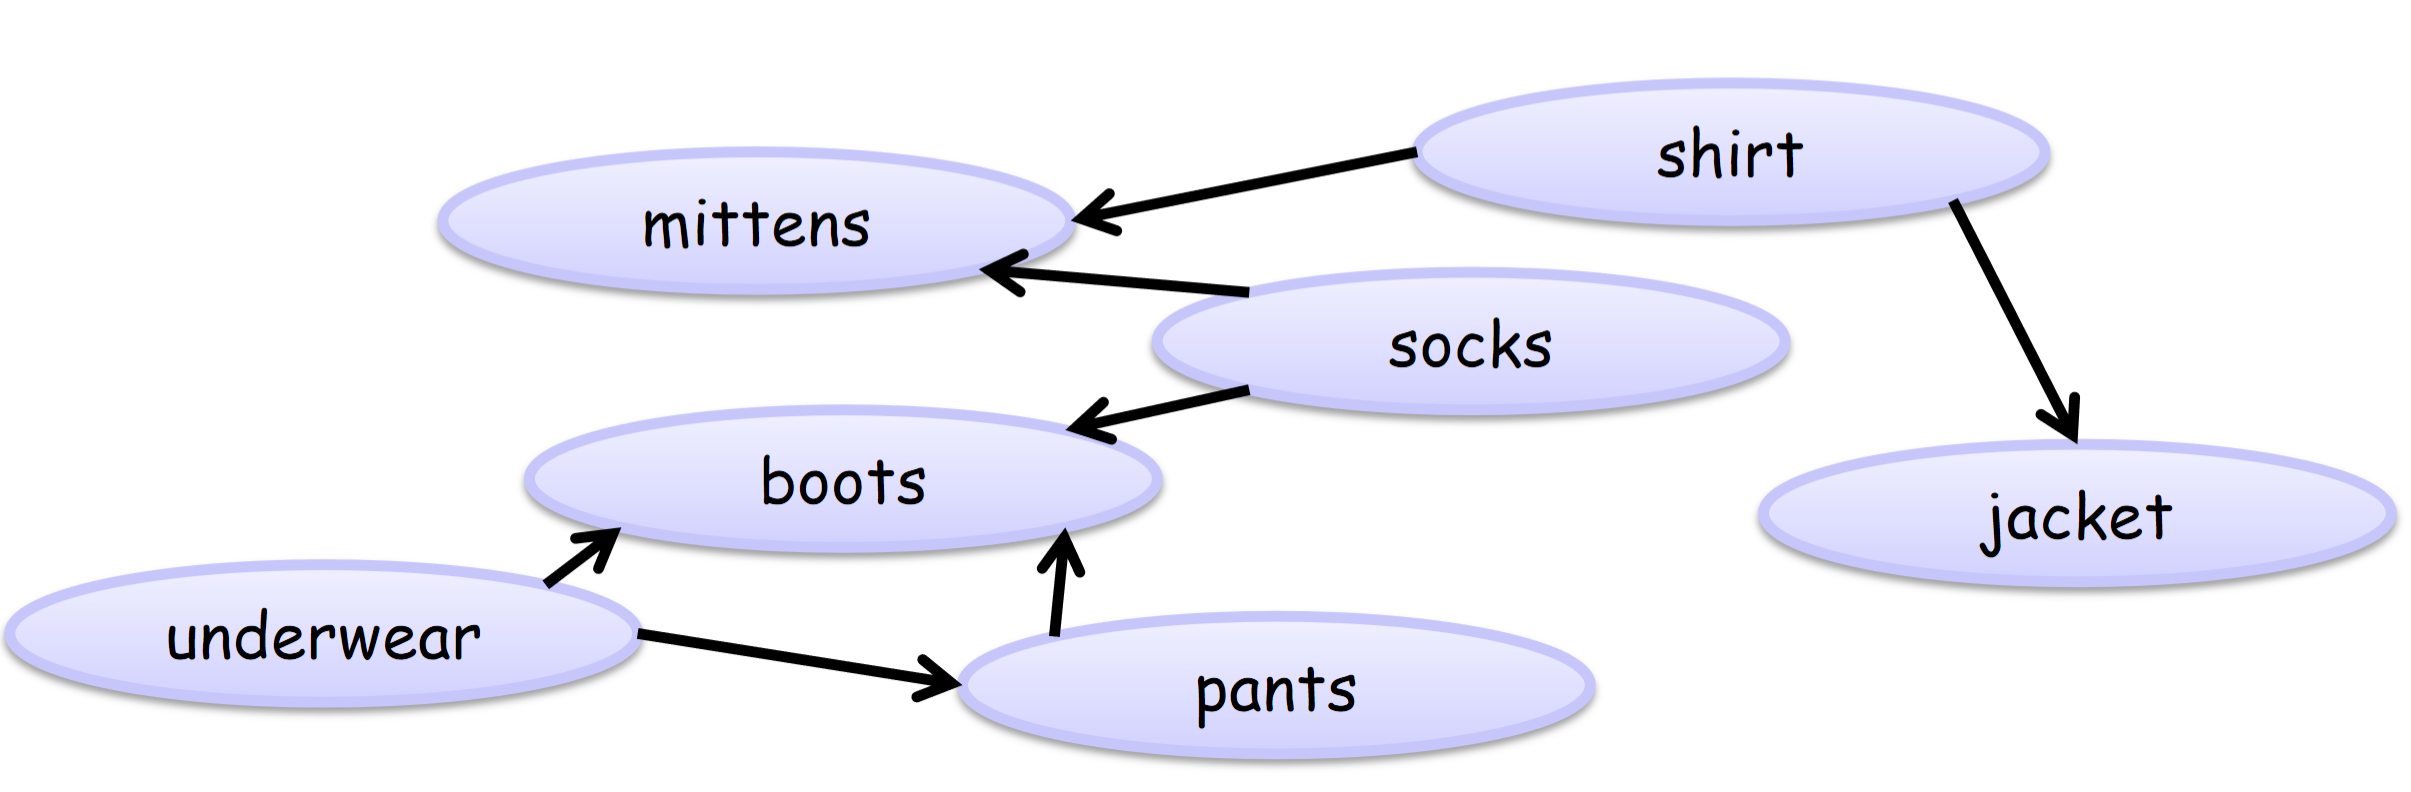
\includegraphics[height=1.5in]{./Sections/graphs/dag/dag.png}
    \end{center}
     \caption{A DAG depicted by getting dressed for winter.}\label{fig:dag}
\end{figure}

\noindent
For each node to be processed its \textbf{dependencies} or parents must be processed first.

\newpage
\begin{Def}[Topological Ordering]

    Given a graph, a \textbf{topological ordering} is a linear ordering of nodes such that for every edge $(u,v)$, $u$ comes before $v$.
\end{Def}

\begin{figure}[h]
    \begin{center}
      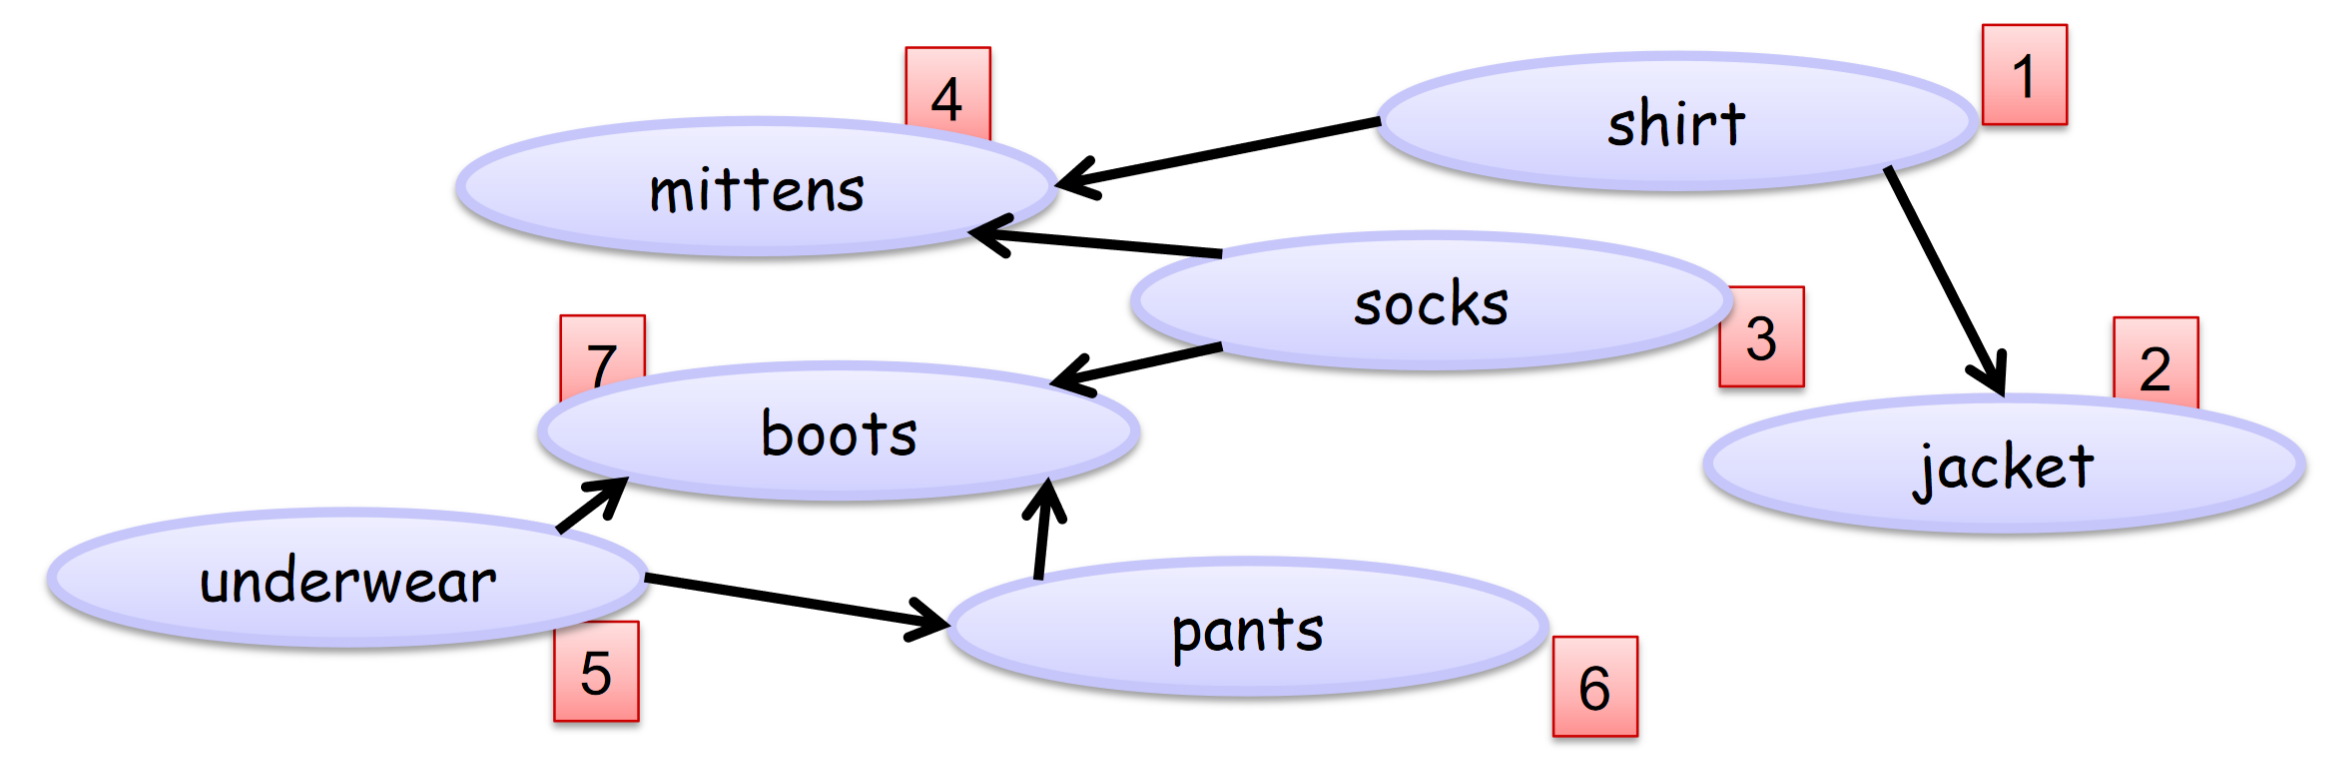
\includegraphics[height=1.5in]{./Sections/graphs/dag/top.png}
    \end{center}
     \caption{A topological ordering of the DAG in Figure (\ref{fig:dag}) enumerated in red.}\label{fig:top}
\end{figure}
\noindent
Another possible ordering of $[1,2,3,4,5,6,7]$ is $[5, 6,1,2,3,4,7]$, as $5\rightarrow 6$ is independent.

\begin{theo}[Topological Sort]
    Given a DAG, a topological ordering can be found.
\end{theo}
\begin{figure}[h]
    \begin{center}
      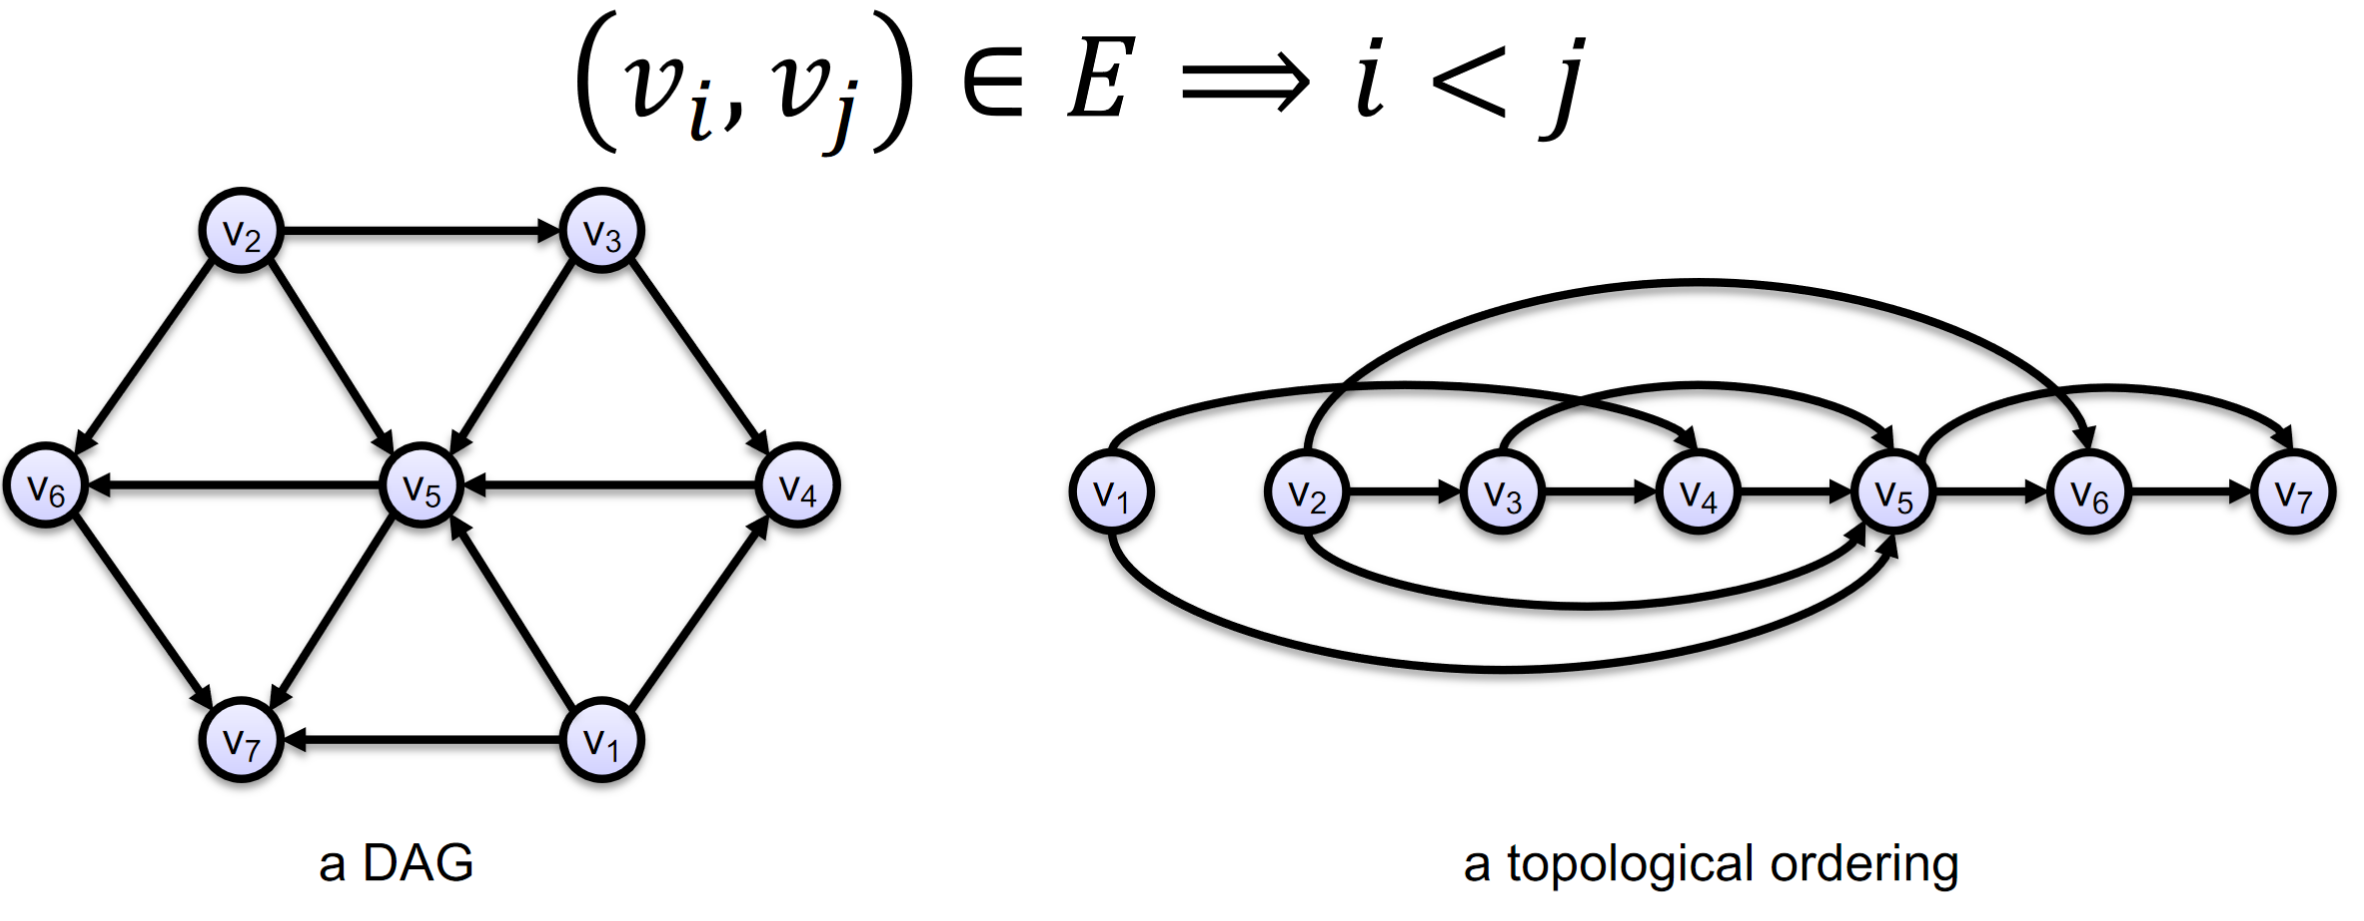
\includegraphics[height=2.5in]{./Sections/graphs/dag/top_sort.png}
    \end{center}
     \caption{A topological sorting of a DAG $E$ and $v$ nodes}\label{fig:top_sort}
\end{figure}
\newpage
\begin{Proof}[Topological Sort via DFS]
    \textit{\textbf{Lemma:}} In a directed graph $G$, if (note necessarily acyclic):
    \begin{itemize}
        \item $(u, v)$ is an edge, and
        \item $v$ is not reachable from $u$,
    \end{itemize}
    Then in every run of DFS, $u.f > v.f$.
    
    \noindent
    \textit{\textbf{Proof:}}
    \begin{itemize}
        \item If $v$ is started before $u$, then the DFS-Visit($v$) will terminate without reaching $u$ (because there is no path to $u$).
        \item If $u$ is started before $v$, then the edge $(u, v)$ will be explored before $u$ is finished.
    \end{itemize}
    Therefore, in all cases, $u.f > v.f$.
\end{Proof}

\begin{Def}[Strongly Connected Components]

    A \textbf{strongly connected component} is a subgraph where every node is reachable from every other node. 
    Then we say $u\rightsquigarrow v$ and $v\rightsquigarrow u$ are \textbf{mutually reachable}. 
\end{Def}

\begin{figure}[h]
    \begin{center}
      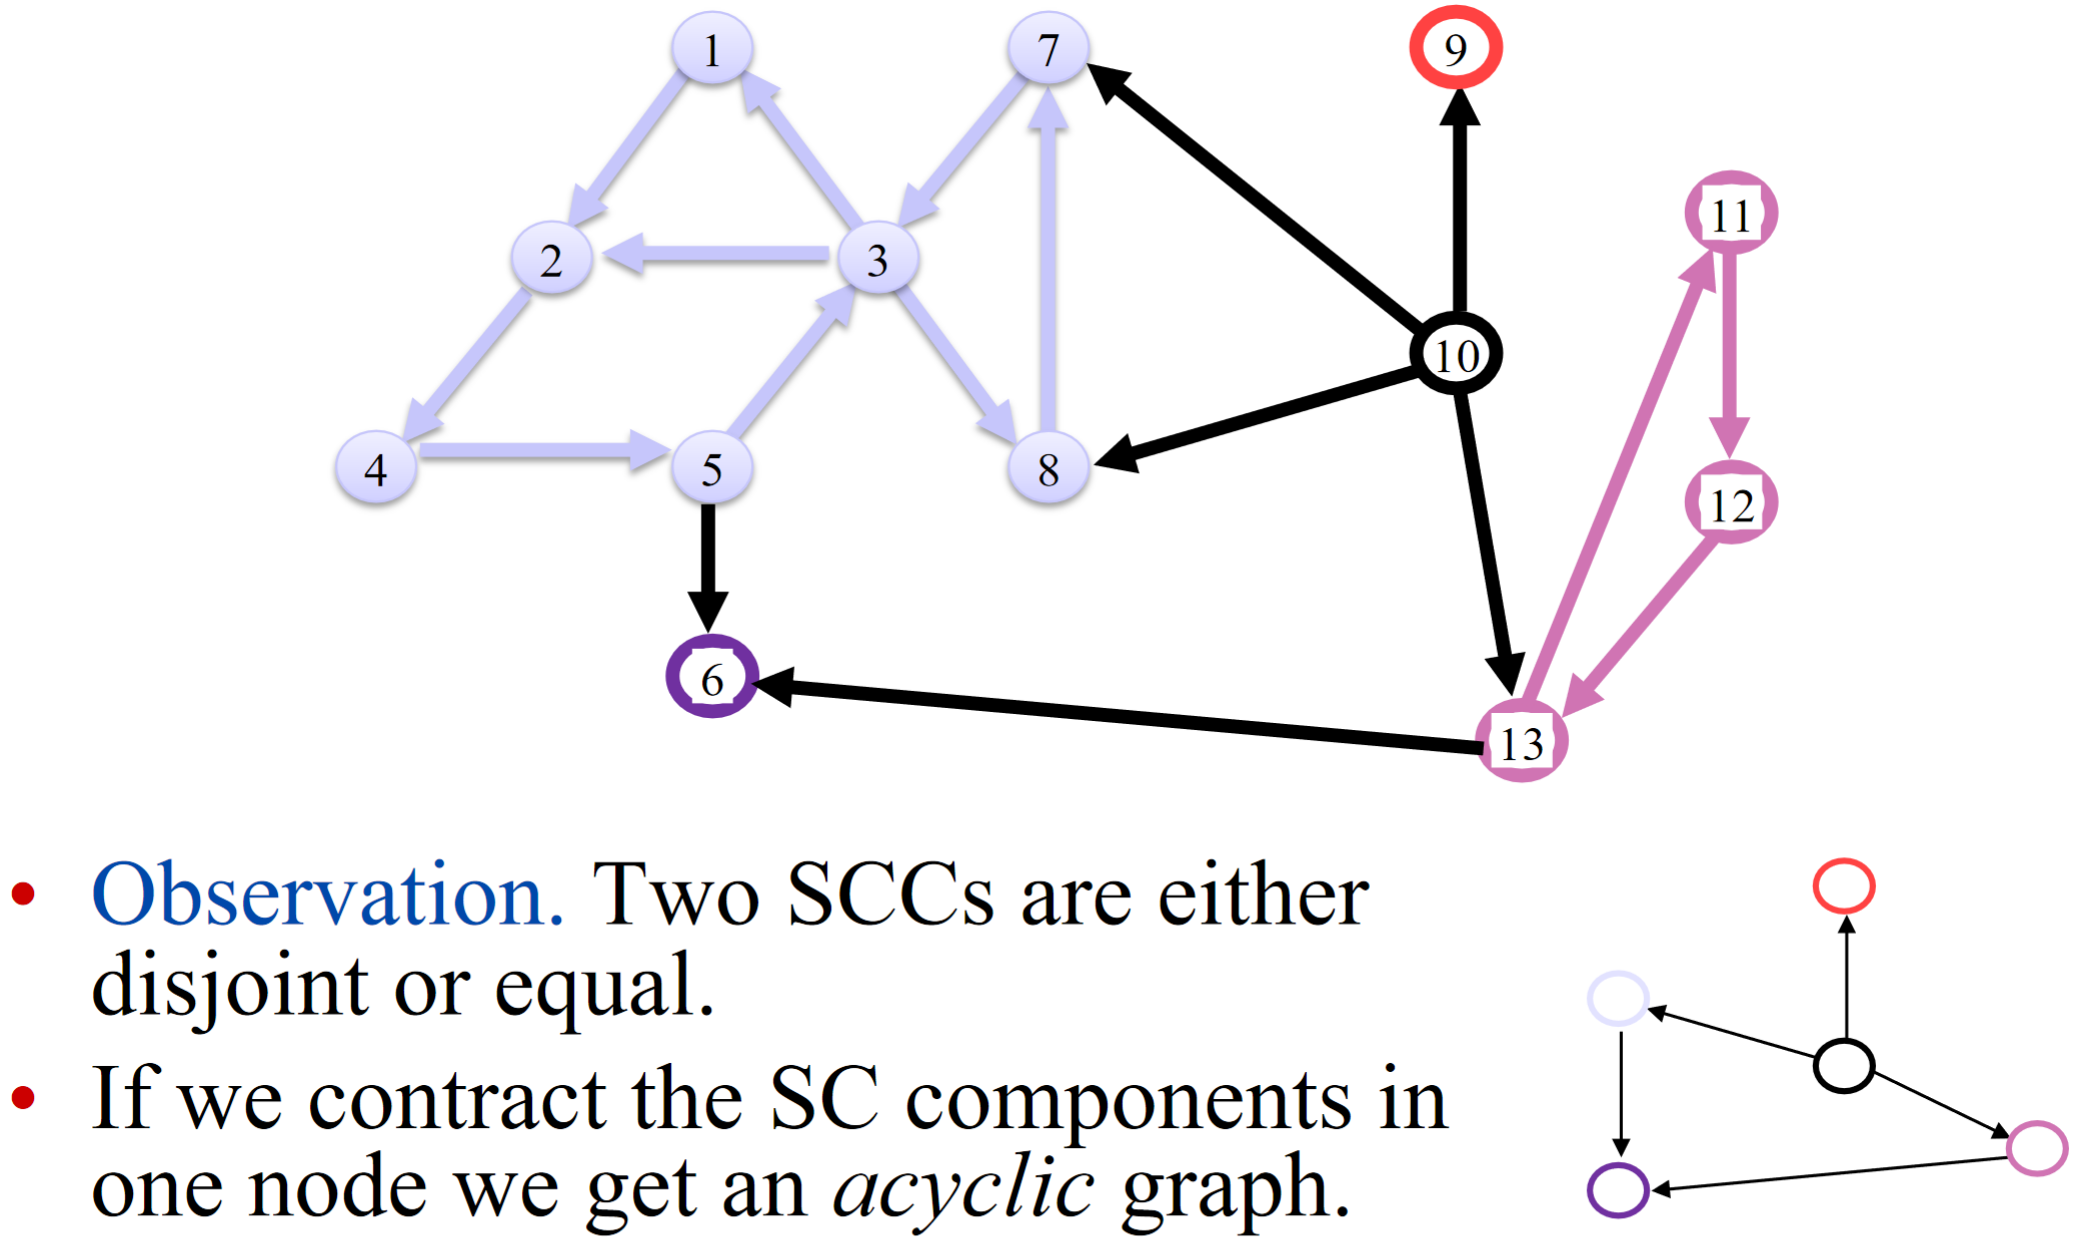
\includegraphics[height=3in]{./Sections/graphs/dag/strong_conn.png}
    \end{center}
     \caption{A graph with 5 strongly connected components.}\label{fig:strong_conn}
\end{figure}